\documentclass[aspectratio=169,11pt]{beamer}
\usepackage[T1]{fontenc}
\usepackage[utf8]{inputenc}
\usepackage{lmodern,amsmath,amssymb,graphicx}
\DeclareUnicodeCharacter{2013}{\ensuremath{-}}
\usetheme{default}
\usefonttheme{serif}
\setbeamercolor{normal text}{fg=black,bg=white}
\setbeamercolor{structure}{fg=black}
\setbeamercolor{frametitle}{fg=black}
\setbeamercolor{title}{fg=black}
\setbeamertemplate{navigation symbols}{}
\setbeamertemplate{footline}[frame number]
\setbeamertemplate{itemize items}[circle]
\setbeamersize{text margin left=8mm,text margin right=8mm}
\setlength{\parskip}{5pt}
\newcommand{\db}{\bar\partial}
\newcommand{\C}{\mathbb C}
\newcommand{\R}{\mathbb R}
\newcommand{\Z}{\mathbb Z}
\newcommand{\A}{\mathcal A}
\newcommand{\F}{\mathcal F}
\newcommand{\Lie}{\mathcal L}
\newcommand{\ee}{e_{n,m}}
\newcommand{\pbarz}{\partial_{\bar z}}
\newcommand{\src}[1]{\par\vfill{\scriptsize #1\par}}
\title{Lecture 13}
\subtitle{Dolbeault's theorem and the $\db$-Poincar\'e lemma}
\author{Daniel Gonz\'alez Casanova Azuela}
\date{}
\hypersetup{pdfauthor={Daniel Gonzalez Casanova Azuela},
 pdftitle={Lecture 13: Dolbeault's theorem and the $\db$-Poincar\'e lemma}}

\begin{document}
\begin{frame}
\titlepage
\end{frame}

\section{Dolbeault's theorem and sheaf cohomology}
\begin{frame}{Dolbeault's theorem: sheaves and sections}
Fix $p$ on a complex manifold $M$. For each open set $U\subset M$,
\[
 \Omega^p_M(U)=\{\text{holomorphic }p\text{-forms on }U\},\qquad
 \A^{p,q}_M(U)=\{\text{smooth }(p,q)\text{-forms on }U\}.
\]
A differential form is a \textbf{section} of a bundle of exterior powers
of the cotangent bundle. Assigning these sections to every open $U$,
with restriction maps, gives its \textbf{sheaf of sections}.

Taking \textbf{global sections} means evaluating the sheaf on $M$:
\[
 \Gamma(M,\A^{p,q}_M)=\A^{p,q}_M(M).
\]
Dolbeault's theorem identifies sheaf cohomology with the cohomology
of the global smooth-form complex:
\[
 \boxed{H^q(M,\Omega^p_M)\cong H^{p,q}_{\db}(M).}
\]
\end{frame}

\begin{frame}{Stalks and exactness}
The \textbf{stalk} $\F_x$ consists of germs $[s]_x$ of sections near $x$.
Two sections have the same germ if they agree on some smaller
neighbourhood of $x$. In particular,
\[
 [s]_x=0
 \quad\Longleftrightarrow\quad
 s|_V=0\ \text{for some neighbourhood }V\text{ of }x.
\]
A complex of sheaves is \textbf{exact at $\mathcal G$} precisely when
\[
 \F\xrightarrow{a}\mathcal G\xrightarrow{b}\mathcal H,
 \qquad
 \ker b_x=\operatorname{im}a_x\quad\text{for every }x.
\]
Thus a section of $\ker b$ must lift through $a$ \textbf{locally near
each point}. Different neighbourhoods may have different lifts.

A \textbf{lift} of $s$ on $V$ means a section $t\in\F(V)$ satisfying
$a(t)=s|_V$.
\end{frame}

\begin{frame}{Sheafification and global sections}
For a sheaf map $\varphi:\F\to\mathcal G$, the image presheaf
\[
 U\longmapsto\operatorname{im}\bigl(\F(U)\xrightarrow{\varphi_U}
 \mathcal G(U)\bigr)
\]
may fail the gluing axiom. Its \textbf{sheafification} is the
\textbf{image sheaf} $\operatorname{im}\varphi$.

A section $s\in\mathcal G(U)$ belongs to this image sheaf precisely
when some open cover $U=\bigcup_i U_i$ admits local lifts:
\[
 t_i\in\F(U_i),\qquad\varphi(t_i)=s|_{U_i}.
\]
The images $s|_{U_i}$ agree on overlaps, but the lifts $t_i$ need not glue.

Thus a \textbf{surjective sheaf map} guarantees local lifts.
The global-sections functor $\Gamma(M,-)$ asks for a lift on all of $M$,
which may not exist. This is why it can fail to be right exact.

\textbf{Sheafification includes sections with local lifts.
It does not guarantee a global lift.}
\end{frame}

\begin{frame}{The $\db$-Poincar\'e lemma on stalks}
Fix $x\in M$ and $q>0$. Take
$[\alpha]_x\in\ker(\db:\A^{p,q}_{M,x}\to\A^{p,q+1}_{M,x})$.
\begin{enumerate}
\item Choose a representative $\alpha$ on a neighbourhood $U$ of $x$.
The equation $[\db\alpha]_x=0$ lets us shrink to $V\subset U$ with
$\db\alpha|_V=0$.
\item The local $\db$-Poincar\'e lemma gives a smaller
$W\subset V$ and a $(p,q-1)$-form $\beta$ with
$\alpha|_W=\db\beta$.
\item Therefore $[\alpha]_x=\db[\beta]_x$.
The reverse inclusion follows from $\db^2=0$.
\end{enumerate}
In degree $0$, $\db\alpha=0$ means that the coefficients of the
$(p,0)$-form $\alpha$ are holomorphic. Hence the sheaf sequence
\[
 0\longrightarrow\Omega^p_M\longrightarrow\A^{p,0}_M
 \xrightarrow{\db}\A^{p,1}_M\xrightarrow{\db}\cdots
\]
is exact: it is a \textbf{resolution of $\Omega^p_M$}.
For $\dim_{\C}M>1$, this uses the several-variable local lemma.
\end{frame}

\begin{frame}{Global sections can lose exactness}
Applying $\Gamma(M,-)$ to the resolution gives the complex
\[
 \A^{p,0}_M(M)\xrightarrow{\db}\A^{p,1}_M(M)
 \xrightarrow{\db}\A^{p,2}_M(M)\longrightarrow\cdots.
\]
For $q>0$, its cohomology is, by definition,
\[
 H^{p,q}_{\db}(M)=
 \frac{\ker(\db:\A^{p,q}_M(M)\to\A^{p,q+1}_M(M))}
 {\operatorname{im}(\db:\A^{p,q-1}_M(M)\to\A^{p,q}_M(M))}.
\]
(Dolbeault cohomology can be nontrivial even coming from an exact
resolution.) Local primitives need not agree on overlaps, so they need not give
a global primitive. The global-sections functor is \textbf{left exact}:
it preserves kernels, but a surjective sheaf map need not be
surjective on global sections.

For example, on our elliptic curve, $d\bar z$ is locally $\db\bar z$
but has no global primitive. Thus $H^{0,1}_{\db}(E)=\C$,
although the sheaf sequence is exact.
\end{frame}

\begin{frame}{The other resolution: the definition of sheaf cohomology}
Work with sheaves of abelian groups.
An \textbf{injective sheaf} $\mathcal I$ has the extension property:
every map $\F'\to\mathcal I$ extends across an inclusion
$\F'\hookrightarrow\F$.

Every sheaf $\F$ admits an \textbf{injective resolution}, an exact
sequence whose terms $\mathcal I^r$ are injective:
\[
 0\longrightarrow\F\longrightarrow\mathcal I^0
 \xrightarrow{d^0}\mathcal I^1\xrightarrow{d^1}\cdots.
\]
Sheaf cohomology is defined by taking global sections first,
then cohomology:
\[
 H^q(M,\F):=R^q\Gamma(M,-)(\F)
 =H^q\bigl(\Gamma(M,\mathcal I^\bullet)\bigr).
\]
Here $R^q\Gamma$ denotes the $q$th right derived functor of $\Gamma$.
The result is independent of the chosen injective resolution,
up to canonical isomorphism.

For Dolbeault's theorem, take $\F=\Omega^p_M$.
\src{Voisin, Chapter 4, Lemma 4.26, Theorem 4.28 and Section 4.3.}
\end{frame}

\begin{frame}{Fine sheaves and acyclic resolutions}
A sheaf $\mathcal G$ is \textbf{acyclic for global sections} if
\[
 H^k(M,\mathcal G)=0\qquad(k>0).
\]
In Voisin's convention, a \textbf{fine sheaf} is a module sheaf over
a ring sheaf admitting locally finite partitions of unity
subordinate to open covers.

The sheaf $\A^{p,r}_M$ is a module over smooth functions.
Partitions of unity act by multiplication:
\[
 \alpha\longmapsto\chi_i\alpha,\qquad
 \sum_i\chi_i\alpha=\alpha.
\]
Thus each $\A^{p,r}_M$ is fine. Proposition 4.36 gives
\[
 H^k(M,\A^{p,r}_M)=0\qquad(k>0,\ \text{every }r).
\]
An \textbf{acyclic resolution} is an exact sheaf resolution whose
individual terms are acyclic. Local exactness comes from
$\db$-Poincar\'e, while acyclicity of the terms comes from fineness.
\src{Voisin, Definitions 4.31 and 4.35, Proposition 4.36.}
\end{frame}

\begin{frame}{Proposition 4.32 and Dolbeault's theorem}
\textbf{Proposition 4.32, for global sections.}
If $0\to\F\to\mathcal C^0\to\mathcal C^1\to\cdots$ is exact and
each $\mathcal C^r$ is acyclic, then
\[
 H^q(M,\F)\cong H^q\bigl(\Gamma(M,\mathcal C^\bullet)\bigr).
\]
For $\F=\Omega^p_M$, compare the Dolbeault and injective resolutions:
\begin{columns}[c,onlytextwidth]
\begin{column}{0.36\textwidth}
\fbox{\parbox[c]{\dimexpr\linewidth-2\fboxsep-2\fboxrule\relax}{
\centering\small
Cohomology of global sections\\
is, by definition, $H^{p,q}_{\db}(M)$.
}}
\end{column}
\begin{column}{0.61\textwidth}
\[
 0\longrightarrow\Omega^p_M\longrightarrow\A^{p,0}_M
 \xrightarrow{\db}\A^{p,1}_M\xrightarrow{\db}\cdots.
\]
\end{column}
\end{columns}

\medskip
\begin{columns}[c,onlytextwidth]
\begin{column}{0.36\textwidth}
\fbox{\parbox[c]{\dimexpr\linewidth-2\fboxsep-2\fboxrule\relax}{
\centering\small
Cohomology of global sections\\
$=H^q(M,\Omega^p_M)$.
}}
\end{column}
\begin{column}{0.61\textwidth}
\[
 0\longrightarrow\Omega^p_M\longrightarrow\mathcal I^0
 \longrightarrow\mathcal I^1\longrightarrow\cdots.
\]
\end{column}
\end{columns}

Both resolutions have acyclic terms, so Proposition 4.32 gives
\[
 \boxed{H^{p,q}_{\db}(M)\cong H^q(M,\Omega^p_M).}
\]
\src{Voisin, Proposition 4.32.}
\end{frame}

\begin{frame}{The homological algebra in degree one}
\textbf{This is how Proposition 4.32 works in the Dolbeault case.}

Let $\mathcal Z^1=\ker(\db:\A^{p,1}_M\to\A^{p,2}_M)$.
The local lemma gives a short exact sequence of sheaves:
\[
 0\longrightarrow\Omega^p_M\longrightarrow\A^{p,0}_M
 \xrightarrow{\db}\mathcal Z^1\longrightarrow0.
\]
Its long exact sequence in sheaf cohomology contains
\[
 \Gamma(M,\A^{p,0}_M)\xrightarrow{\db}\Gamma(M,\mathcal Z^1)
 \longrightarrow H^1(M,\Omega^p_M)
 \longrightarrow H^1(M,\A^{p,0}_M)=0.
\]
The final vanishing uses \textbf{fineness}. Exactness therefore gives
\[
 H^1(M,\Omega^p_M)\cong
 \frac{\Gamma(M,\mathcal Z^1)}
 {\db\,\Gamma(M,\A^{p,0}_M)}
 =H^{p,1}_{\db}(M).
\]
The numerator consists of global closed forms, and the denominator
of global exact forms. Repeating this argument with the successive
kernel sheaves proves the comparison in higher degrees.
\end{frame}

\begin{frame}{Pierre Dolbeault}
\centering
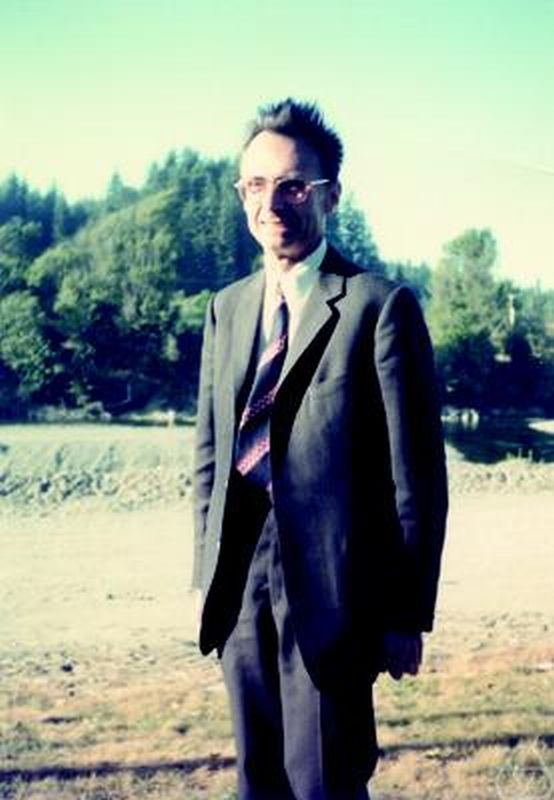
\includegraphics[width=0.9\textwidth,height=6cm,keepaspectratio]{../assets/Pierre_Dolbeault.jpg}
\end{frame}

\begin{frame}{Pending computation: $L^2$ closure}
For $A=\operatorname{span}\{e^{int}:n\in\Z\}\subset C(S^1,\C)$,
the hypotheses hold:
\begin{itemize}
\item $A$ is an algebra, since $e^{int}e^{imt}=e^{i(n+m)t}$;
\item $1=e^{i0t}\in A$;
\item $A$ is closed under conjugation, since
      $\overline{e^{int}}=e^{-int}$;
\item $A$ separates points of $S^1$: the function $e^{it}$ already does.
\end{itemize}
Therefore Stone--Weierstrass gives
\[
 \overline A^{\,\|\cdot\|_\infty}=C(S^1,\C).
\]
\end{frame}

\begin{frame}{Uniform convergence implies $L^2$ convergence}
Take $f\in C(S^1,\C)$. By Stone--Weierstrass there are
$p_n\in A$ such that
\[
\|p_n-f\|_\infty\longrightarrow0.
\]
Since $S^1$ has finite volume,
\[
\begin{aligned}
\|p_n-f\|_{L^2}^2
&=\int_{S^1}|p_n-f|^2\\
&\le \int_{S^1}\|p_n-f\|_\infty^2\\
&=\operatorname{vol}(S^1)\,\|p_n-f\|_\infty^2.
\end{aligned}
\]
Therefore
\[
\boxed{
\|p_n-f\|_{L^2}
\le \sqrt{\operatorname{vol}(S^1)}\,\|p_n-f\|_\infty
\longrightarrow0.
}
\]
Thus
\[
\boxed{C(S^1,\C)\subseteq\overline A^{\,L^2}.}
\]
\end{frame}

\begin{frame}{From continuous functions to all of $L^2$}
We have proved
\[
C(S^1,\C)\subseteq\overline A^{\,L^2}.
\]
Now use the separate fact that continuous functions are dense in $L^2(S^1)$
(Folland, Proposition~7.9). Since $S^1$ is compact,
\[
\overline{C(S^1,\C)}^{\,L^2}=L^2(S^1).
\]
Since $\overline A^{\,L^2}$ is already closed and contains
$C(S^1,\C)$, it must contain its $L^2$-closure. Hence
\[
L^2(S^1)
\subseteq \overline A^{\,L^2}.
\]
The reverse inclusion is automatic because $A\subset L^2(S^1)$.
Therefore
\[
\boxed{\overline A^{\,L^2}=L^2(S^1).}
\]
So the Fourier modes are complete in $L^2(S^1)$.
\src{Folland, \emph{Real Analysis}, 2nd ed., Proposition~7.9.}
\end{frame}

\section{Reminder: the one-variable solution}

\begin{frame}{Reminder: the Fourier solution, now called $P$}
Last lecture, we solved the nonconstant Fourier modes on
$E=\C/(2\pi\Z+2\pi i\Z)$. Recall
\[
 e_{n,m}=e^{inx+imy},\qquad
 \partial_{\bar z}e_{n,m}=\frac{in-m}{2}e_{n,m}.
\]
For a smooth function $g=\sum_{n,m}g_{n,m}e_{n,m}$, we now give that
construction the name $P$:
\[
 Pg=\sum_{(n,m)\ne(0,0)}\frac{2g_{n,m}}{in-m}e_{n,m}.
\]
Differentiating cancels each denominator, so
\[
 \boxed{\partial_{\bar z}Pg=g-g_{0,0}.}
\]
The constant $g_{0,0}=\frac{1}{(2\pi)^2}\int_E g\,dx\,dy$ is the average of $g$.
Smooth Fourier coefficients decay rapidly, so the series and all its
derivatives converge.
\src{Lecture 12 recap. The operator name $P$ is new notation.}
\end{frame}

\begin{frame}{When may we differentiate an infinite sum?}
\setlength{\parskip}{3pt}
\setlength{\abovedisplayskip}{4pt}
\setlength{\belowdisplayskip}{4pt}
The given $g$ is already smooth. We must justify differentiating
the infinite series defining $Pg$.

\textbf{Differentiation criterion.}
For smooth terms $u_{n,m}$ on the torus, if the three series
\[
 \sum_{n,m}u_{n,m},\qquad
 \sum_{n,m}\partial_xu_{n,m},\qquad
 \sum_{n,m}\partial_yu_{n,m}
\]
converge uniformly, their sum is $C^1$, and we may differentiate term by term.
To prove smoothness, repeat this for every derivative order.

\textbf{Weierstrass M-test.}
A series converges uniformly if its terms satisfy
\[
 |u_{n,m}(x,y)|\le M_{n,m}\quad\hbox{at every point},\qquad
 \sum_{n,m}M_{n,m}<\infty.
\]
\textbf{Uniformly} means that the same tail bound works at every point.
We apply this test to the original series and to each derivative series.
The next slide supplies the Fourier coefficient bounds.
\end{frame}

\begin{frame}{Why smoothness makes Fourier coefficients small: $x$}
\setlength{\abovedisplayskip}{4pt}
\setlength{\belowdisplayskip}{4pt}

Keep $y$ fixed. Integration by parts gives
\[
 \int_0^{2\pi}g_x e^{-inx}\,dx
 =\underbrace{[g e^{-inx}]_0^{2\pi}}_{0\ \text{by periodicity}}
   +in\int_0^{2\pi}g e^{-inx}\,dx.
\]
Multiply by $e^{-imy}$, integrate in $y$, and divide by $(2\pi)^2$.
Since
\[
g_{n,m}=\frac{1}{(2\pi)^2}\int_E g(x,y)e^{-inx-imy}
       =\langle g,e_{n,m}\rangle,
\]
we get
\[
(g_x)_{n,m}=in\,g_{n,m}.
\]
Applying the same identity repeatedly,
\[
\boxed{(g_{xxxx})_{n,m}=(in)^4g_{n,m}=n^4g_{n,m}.}
\]
Since $g_{xxxx}$ is bounded on the compact torus, say by $C_x$,
\[
\boxed{|g_{n,m}|\le \frac{C_x}{|n|^4}\qquad(n\ne0).}
\]
\end{frame}

\begin{frame}{The same estimate in $y$}
\setlength{\abovedisplayskip}{5pt}
\setlength{\belowdisplayskip}{5pt}

Repeat the whole calculation with $x$ and $y$ interchanged.
Integration by parts in $y$ gives
\[
(g_y)_{n,m}=im\,g_{n,m}.
\]
Applying this four times,
\[
\boxed{(g_{yyyy})_{n,m}=(im)^4g_{n,m}=m^4g_{n,m}.}
\]
Since $g_{yyyy}$ is bounded on the compact torus, say by $C_y$,
its Fourier coefficients have absolute value at most $C_y$. Therefore
\[
m^4|g_{n,m}|\le C_y
\quad\Longrightarrow\quad
\boxed{|g_{n,m}|\le\frac{C_y}{|m|^4}\qquad(m\ne0).}
\]
\end{frame}

\begin{frame}{Combining the two estimates}
For $(n,m)\ne(0,0)$, set
\[
k=\max(|n|,|m|).
\]
Then either $|n|=k$ or $|m|=k$. Hence, with
\[
C=\max(C_x,C_y),
\]
the two previous estimates give
\[
\boxed{|g_{n,m}|\le \frac{C}{k^4}.}
\]

Now group the Fourier series into square shells:
\[
S_k:=\{(n,m)\in\mathbb Z^2:\max(|n|,|m|)=k\},
\]
so that
\[
\sum_{(n,m)\in\mathbb Z^2}g_{n,m}e_{n,m}
=
g_{0,0}
+\sum_{k=1}^{\infty}
\sum_{(n,m)\in S_k}g_{n,m}e_{n,m}.
\]
\end{frame}

\begin{frame}{How many modes are in one shell?}
Each $S_k$ is the boundary of the lattice square $[-k,k]^2$.

Its side length is $2k$. Along each of the four sides there are
$2k$ new lattice steps, so
\[
\boxed{|S_k|=8k.}
\]

Therefore, using $|g_{n,m}|\le C/k^4$ on $S_k$,
\[
\sum_{(n,m)\in S_k}|g_{n,m}|
\le 8k\,\frac{C}{k^4}
=\frac{8C}{k^3}.
\]
Hence
\[
\sum_{(n,m)\ne(0,0)}|g_{n,m}|
\le 8C\sum_{k=1}^{\infty}\frac1{k^3}<\infty.
\]
By the Weierstrass M-test, the Fourier series converges uniformly.
This is the kind of uniform convergence required by the Zorich
termwise-differentiation criterion.
\end{frame}





\begin{frame}{Why four derivatives are enough}
Differentiate one Fourier term:
\[
\partial_x\bigl(g_{n,m}e_{n,m}\bigr)
=in\,g_{n,m}e_{n,m},
\]
and similarly for $\partial_y$.

On $S_k$, $|n|,|m|\le k$, so one derivative costs at most one factor $k$.
Thus
\[
\sum_{(n,m)\in S_k}
|\partial_x(g_{n,m}e_{n,m})|
\le
8k\cdot k\cdot\frac{C}{k^4}
=
\frac{8C}{k^2}.
\]
Since
\[
\sum_{k=1}^{\infty}\frac1{k^2}<\infty,
\]
the derivative series converges uniformly by the M-test.

Therefore the termwise-differentiation criterion applies.
\end{frame}

\begin{frame}{Reminder: $T$ produces a local primitive}
\setlength{\parskip}{3pt}
\setlength{\abovedisplayskip}{4pt}
\setlength{\belowdisplayskip}{4pt}
Choose disks $\overline D\subset D^+$ inside a fundamental square of $E$
(after rescaling).
Fix a \textbf{bump function} $\chi$ supported in $D^+$ and equal to $1$
near $\overline D$.

For $g\in C^\infty(D^+)$, extend $\widetilde g=\chi g$ by zero to $E$. Write
\[
 c=\frac1{(2\pi)^2}\int_E\widetilde g\,dx\,dy,\qquad
 Tg=(P\widetilde g)|_D+c\bar z.
\]
The Fourier formula gives $\partial_{\bar z}P\widetilde g=\widetilde g-c$.
Consequently,
\[
 \boxed{\partial_{\bar z}(Tg)=g
 \quad\Longleftrightarrow\quad
 \db(Tg)=g\,d\bar z}\qquad\hbox{on }D.
\]
We use the same $\chi$ for every $g$, so $T$ is linear.

\[
 \boxed{
 g\ \text{smooth function}
 \quad\overset{T}{\longmapsto}\quad
 Tg\ \text{a primitive of }g\,d\bar z
 }
\]

On the torus, $\bar z$ is not a global function.
On the disk it is available and removes the constant term.
\end{frame}

\begin{frame}{Using $T$ with the other variables as parameters}
For today's proof, let $g=g(z_1,\ldots,z_n)$ be smooth.
Write $T_i$ for applying $T$ only in $z_i$, with the other coordinates
as parameters. On a smaller polydisk,
\[
 \partial_{\bar z_i}(T_i g)=g.
\]
Use the same bump function in $z_i$ for every value of the parameters.
Multiplication by this function, the Fourier coefficients, and the average
all operate only in $z_i$. Therefore, for $j\ne i$,
\[
 \partial_{\bar z_j}(T_i g)=T_i(\partial_{\bar z_j}g).
\]
Rapid Fourier decay on compact sets of parameters justifies differentiation.
In particular,
\[
 \partial_{\bar z_j}g=0\quad\Longrightarrow\quad
 \partial_{\bar z_j}(T_i g)=0.
\]
\textbf{Solving in one variable preserves holomorphic dependence
on the other variables.}
\end{frame}

\section{Today's proof outline}

\begin{frame}{Today's proof outline}
\textbf{Goal.} For a closed $(p,q)$-form $\eta$ with $q>0$, find a
primitive $\eta=\db\beta$ near each point.
\begin{enumerate}
\item \textbf{Solve in the first variable.}
Use $T_1$ to choose a correction $\beta_1$ so that
$\eta-\db\beta_1$ has no $d\bar z_1$ term.

\item \textbf{Use closedness.}
The remainder's coefficients are holomorphic in $z_1$.
Solving in the next variable preserves this property, so the next
correction keeps the first direction removed.

\item \textbf{Repeat.}
After all $n$ directions, no $d\bar z_i$ remains.
A form with $q>0$ must then be zero.
Adding the corrections gives the primitive.
\end{enumerate}
We will work this out for $\alpha=a\,d\bar z_1+b\,d\bar z_2$ on a bidisk.
A bidisk is a product of two disks. We can shrink it during the proof.
\end{frame}

\section{The two-variable example}

\begin{frame}{Two variables: what are we trying to solve?}
Let
\[
 \alpha=a\,d\bar z_1+b\,d\bar z_2
\]
be a smooth $(0,1)$-form on a bidisk, with $\db\alpha=0$.
The coefficients $a,b$ may depend on both coordinates and their conjugates.

We want a function $u$ such that
\[
 \db u=(\partial_{\bar z_1}u)\,d\bar z_1
       +(\partial_{\bar z_2}u)\,d\bar z_2=\alpha.
\]
Equivalently, we want to solve both equations
\[
 \boxed{\partial_{\bar z_1}u=a,\qquad\partial_{\bar z_2}u=b.}
\]
We allow a smaller bidisk at each use of the one-variable operator.
\end{frame}

\begin{frame}{First correction: removing the $d\bar z_1$ term}
\textbf{We will construct $u$ as $u_1+u_2$.}

Apply the one-variable operator in $z_1$, with $z_2$ as a parameter:
\[
 u_1=T_1a,\qquad \partial_{\bar z_1}u_1=a.
\]
Its full Dolbeault derivative is
\[
 \db u_1=a\,d\bar z_1+(\partial_{\bar z_2}u_1)\,d\bar z_2.
\]
Subtracting it gives
\[
 \boxed{\alpha-\db u_1=r\,d\bar z_2,\qquad
 r=b-\partial_{\bar z_2}u_1.}
\]
\textbf{The first coefficient is now correct.}
The remaining task is to find $u_2$ with
\[
 \partial_{\bar z_2}u_2=r,\qquad \partial_{\bar z_1}u_2=0.
\]
The second condition ensures that adding $u_2$ keeps the first equation solved.
\end{frame}

\begin{frame}{What must the remainder satisfy?}
To keep the first equation solved when we set $u_2=T_2r$,
we want $\partial_{\bar z_1}r=0$.

Recall $r=b-\partial_{\bar z_2}u_1$ and $\partial_{\bar z_1}u_1=a$.
Compute, using commutativity of mixed derivatives:
\[
 \begin{aligned}
 \partial_{\bar z_1}r
 &=\partial_{\bar z_1}b
   -\partial_{\bar z_1}\partial_{\bar z_2}u_1\\
 &=\partial_{\bar z_1}b
   -\partial_{\bar z_2}\partial_{\bar z_1}u_1\\
 &=\partial_{\bar z_1}b-\partial_{\bar z_2}a.
 \end{aligned}
\]
Thus the condition we need is
\[
 \partial_{\bar z_1}b=\partial_{\bar z_2}a.
\]
\textbf{Now we use the assumption $\db\alpha=0$.}
\end{frame}

\begin{frame}{Closedness gives exactly what we need}
For $\alpha=a\,d\bar z_1+b\,d\bar z_2$, expand
\[
 \begin{aligned}
 \db\alpha
 &=\db a\wedge d\bar z_1+\db b\wedge d\bar z_2\\
 &=(\partial_{\bar z_2}a)\,d\bar z_2\wedge d\bar z_1
  +(\partial_{\bar z_1}b)\,d\bar z_1\wedge d\bar z_2\\
 &=\bigl(\partial_{\bar z_1}b-\partial_{\bar z_2}a\bigr)
       d\bar z_1\wedge d\bar z_2.
 \end{aligned}
\]
Here we used
\[
 d\bar z_i\wedge d\bar z_i=0,\qquad
 d\bar z_2\wedge d\bar z_1=-d\bar z_1\wedge d\bar z_2.
\]
The basis form $d\bar z_1\wedge d\bar z_2$ is nonzero. Hence
\[
 \boxed{\db\alpha=0\quad\Longleftrightarrow\quad
 \partial_{\bar z_1}b=\partial_{\bar z_2}a.}
\]
\textbf{This is precisely the compatibility condition we need!}
Since $\db\alpha=0$, the difference we just computed vanishes:
$\partial_{\bar z_1}r=0$.
Thus $r$ is holomorphic in $z_1$, though it may depend on $\bar z_2$.
\end{frame}

\begin{frame}{Second correction: keeping the first equation solved}
Solve in $z_2$:
\[
 u_2=T_2r,\qquad \partial_{\bar z_2}u_2=r.
\]
Applying $T_2$ preserves \textbf{being holomorphic in $z_1$}:
its integrals and Fourier sums use weights independent of $z_1$.
Since $\partial_{\bar z_1}r=0$,
\[
 \partial_{\bar z_1}u_2
 =\partial_{\bar z_1}(T_2r)
 =T_2(\partial_{\bar z_1}r)=T_2(0)=0.
\]
Thus $\db u_2=r\,d\bar z_2$, and
\[
 \boxed{\alpha=\db u_1+r\,d\bar z_2=\db(u_1+u_2).}
\]
Closedness made $r$ holomorphic in $z_1$, and $T_2$ preserved this.
Thus the second correction kept the first equation solved.
\end{frame}

\section{The same corrections in \texorpdfstring{$n$}{n} variables}

\begin{frame}{$n$ variables: one equation for each coefficient}
Let $\alpha$ be a smooth, $\db$-closed $(0,1)$-form near a point:
\[
 \alpha=\sum_{j=1}^n a_j\,d\bar z_j.
\]
Finding a function $u$ with $\db u=\alpha$ means solving
\[
 \partial_{\bar z_1}u=a_1,\quad
 \partial_{\bar z_2}u=a_2,\quad\ldots,\quad
 \partial_{\bar z_n}u=a_n.
\]
\textbf{We will construct $u=u_1+\cdots+u_n$.}
The correction $u_k$ will fix equation $k$ while keeping equations
$1,\ldots,k-1$ solved.

Choose a polydisk around the point inside the given neighbourhood.
At each step we may shrink it, keeping the point inside.
There are only $n$ steps.
\src{Misha's Lecture 13, slides 5--10: the $\db$-Poincar\'e lemma.
Here we write the proof using successive coordinate corrections.}
\end{frame}

\begin{frame}{What remains after the first $k-1$ corrections?}
Suppose we have already removed the terms containing
$d\bar z_1,\ldots,d\bar z_{k-1}$. Write the remainder as
\[
 R_{k-1}
 :=\alpha-\db(u_1+\cdots+u_{k-1})
 =\sum_{j=k}^n r_j\,d\bar z_j.
\]
The functions $r_j$ are the \textbf{current errors}.
At the $k$th step we want a correction $u_k$ satisfying
\[
 \partial_{\bar z_k}u_k=r_k,
 \qquad
 \partial_{\bar z_i}u_k=0\quad(i<k).
\]
The latter condition means that adding $u_k$ keeps all the previous
equations solved.

The remainder is still closed:
\[
 \db R_{k-1}
 =\underbrace{\db\alpha}_{0}
  -\underbrace{\db^2(u_1+\cdots+u_{k-1})}_{0}=0.
\]
For $k=1$, no correction has been made yet:
$R_0=\alpha$ and $r_j=a_j$.

Next we check why solving the $k$th equation will preserve the earlier ones.
\end{frame}

\begin{frame}{Closedness gives the same compatibility equation}
For any $(0,1)$-form
\[
 R=\sum_{\ell=1}^n c_\ell\,d\bar z_\ell,
\]
the coefficient of $d\bar z_i\wedge d\bar z_j$ in $\db R$ is
\[
 \partial_{\bar z_i}c_j-\partial_{\bar z_j}c_i.
\]
Therefore
\[
 \db R=0
 \quad\Longrightarrow\quad
 \boxed{\partial_{\bar z_i}c_j
 =\partial_{\bar z_j}c_i.}
\]

This is exactly the equation from the two-variable case:
\[
 \partial_{\bar z_1}b=\partial_{\bar z_2}a.
\]

Now apply it to the current remainder $R_{k-1}$.
\end{frame}

\begin{frame}{Apply the compatibility equation to the remainder}
Recall
\[
 R_{k-1}=\sum_{j=k}^n r_j\,d\bar z_j.
\]
Take an earlier index $i<k$ and a remaining index $j\ge k$.

The coefficient of $d\bar z_i$ in $R_{k-1}$ is already $0$,
because the $i$th equation has been solved.
So in the compatibility equation,
\[
 c_i=0,\qquad c_j=r_j.
\]
Hence closedness gives
\[
 \partial_{\bar z_i}r_j
 =\partial_{\bar z_j}(0)=0.
\]
Therefore
\[
 \boxed{\partial_{\bar z_i}r_j=0
 \qquad(i<k,\ j\ge k).}
\]

{\bf So every remaining error is holomorphic in each variable
whose equation has already been solved.}
\end{frame}

\begin{frame}{The $k$th correction}
Apply $T$ in the $k$th variable to the current error:
\[
 u_k:=T_k r_k.
\]
Then
\[
 \partial_{\bar z_k}u_k=r_k.
\]
And for every earlier index $i<k$,
\[
 \partial_{\bar z_i}u_k
 =\partial_{\bar z_i}(T_k r_k)
 =T_k(\partial_{\bar z_i}r_k)
 =T_k(0)=0.
\]
Thus
\[
 \boxed{
 \partial_{\bar z_k}u_k=r_k,
 \qquad
 \partial_{\bar z_i}u_k=0\quad(i<k).
 }
\]

The first equation fixes the $k$th error.
The second says that this correction keeps all previous equations solved.
\end{frame}

\begin{frame}{After $n$ corrections, every equation is solved}
Recall we had
\[
 R_{k-1}:=\alpha-\db(u_1+\cdots+u_{k-1})
 =\sum_{j=k}^n r_j\,d\bar z_j.
\]
Now subtract the correction just constructed:
\[
 R_k:=R_{k-1}-\db u_k
 =\sum_{j=k+1}^n
   \bigl(r_j-\partial_{\bar z_j}u_k\bigr)\,d\bar z_j.
\]
There is now no term in $d\bar z_1,\ldots,d\bar z_k$.
Also $\db R_k=0$, because we subtracted an exact form.
So we can apply the same argument to $R_k$.
After the $n$th step there are no coefficients left:
\[
 R_n=0.
\]
By the definition of the remainders,
\[
 \boxed{\alpha=\db(u_1+\cdots+u_n).}
\]
All the corrections restrict to the final, smaller polydisk.
This proves the $\db$-Poincar\'e lemma for $(0,1)$-forms in any dimension.
\end{frame}

\section{Higher-degree forms}

\begin{frame}{General $(0,q)$: the same induction}
The $(0,1)$ proof already contains the whole pattern.

After the first $k-1$ corrections, assume we have a closed remainder
$R_{k-1}$ such that
\[
\boxed{
\begin{array}{l}
R_{k-1}\text{ has no factor }d\bar z_1,\ldots,d\bar z_{k-1},\\[2pt]
\text{its coefficients are holomorphic in }z_1,\ldots,z_{k-1}.
\end{array}}
\]
This is the same induction hypothesis as before.

Now separate the terms containing $d\bar z_k$:
\[
R_{k-1}=d\bar z_k\wedge B+C,
\qquad
B=\sum_J b_J\,d\bar z_J.
\]
Define the $k$th correction by applying $T_k$ coefficientwise:
\[
\boxed{\beta_k:=T_kB=\sum_J(T_kb_J)\,d\bar z_J.}
\]
\end{frame}

\begin{frame}{General $(0,q)$: the $k$th correction}
Exactly as before, $T_k$ solves the $k$th equation:
\[
\begin{aligned}
\db\beta_k
&=\sum_J\sum_{i=1}^n
 \partial_{\bar z_i}(T_kb_J)\,
 d\bar z_i\wedge d\bar z_J\\
&=d\bar z_k\wedge B
 +\sum_J\sum_{i\ne k}
 \partial_{\bar z_i}(T_kb_J)\,
 d\bar z_i\wedge d\bar z_J,
\end{aligned}
\]
because $\partial_{\bar z_k}(T_kb_J)=b_J$.

For every earlier $i<k$,
\[
\partial_{\bar z_i}(T_kb_J)
=T_k(\partial_{\bar z_i}b_J)=0,
\]
by the induction hypothesis.

So $\db\beta_k$ removes the $d\bar z_k$ terms and does not
reintroduce any of the earlier factors.
\end{frame}

\begin{frame}{General $(0,q)$: the new remainder}
Now do exactly what we did for $(0,1)$:
\[
\boxed{R_k:=R_{k-1}-\db\beta_k.}
\]
We have just proved that $R_k$ has no factor
\[
d\bar z_1,\ldots,d\bar z_k.
\]
It is still closed:
\[
\db R_k
=\underbrace{\db R_{k-1}}_{0}
 -\underbrace{\db^2\beta_k}_{0}
=0.
\]

Now closedness gives the same compatibility conclusion as before:
since the $d\bar z_i$ factors for $i\le k$ are absent,
the remaining coefficients must satisfy
\[
\boxed{\partial_{\bar z_i}r_J=0\qquad(i\le k).}
\]
Thus they are holomorphic in $z_1,\ldots,z_k$.

\textbf{So $R_k$ satisfies the same induction hypothesis with $k$
in place of $k-1$.}
\end{frame}

\begin{frame}{After the last correction}
Repeat the same step for $k=1,\ldots,n$:
\[
R_{k-1}\longmapsto
R_k:=R_{k-1}-\db\beta_k.
\]
After step $k$, the remainder has no factor
$d\bar z_1,\ldots,d\bar z_k$.

After the $n$th step, no $d\bar z_j$ factor is available.
Since $q>0$, every term of a $(0,q)$-form needs at least one such factor.
Therefore
\[
\boxed{R_n=0.}
\]
Since
\[
R_n
=\alpha-\db(\beta_1+\cdots+\beta_n),
\]
we obtain
\[
\boxed{\alpha=\db(\beta_1+\cdots+\beta_n).}
\]
\end{frame}

\begin{frame}{Including the $dz_i$ factors: general $(p,q)$}
In coordinates, write
\[
 \eta=\sum_I dz_I\wedge\alpha_I,
 \qquad dz_I=dz_{i_1}\wedge\cdots\wedge dz_{i_p}.
\]
Here $I=(i_1<\cdots<i_p)$ and each $\alpha_I$ is a $(0,q)$-form.
Since $\db(dz_I)=0$, the product rule gives
\[
 0=\db\eta=(-1)^p\sum_I dz_I\wedge\db\alpha_I.
\]
The sign comes from passing the differential across the $p$ factors
$dz_{i_1},\ldots,dz_{i_p}$.

Terms with different $I$ have different $dz$ factors, so they cannot
cancel. Thus $\db\alpha_I=0$ for each $I$.

\textbf{We can solve each of these $(0,q)$-forms using the result
we just proved.}
\end{frame}

\begin{frame}{The primitive for a general $(p,q)$-form}
For each coefficient form in $\eta=\sum_I dz_I\wedge\alpha_I$,
choose a $(0,q-1)$-form $\gamma_I$ satisfying
\[
 \db\gamma_I=\alpha_I.
\]
There are finitely many $I$, so we can take a common smaller polydisk
where all these equations hold.

Put the $dz_I$ factors back, with the sign from the product rule:
\[
 \beta:=(-1)^p\sum_I dz_I\wedge\gamma_I.
\]
This is a $(p,q-1)$-form. Differentiating, the two signs cancel:
\[
 \boxed{\db\beta=(-1)^p(-1)^p
       \sum_I dz_I\wedge\db\gamma_I=\eta.}
\]
\end{frame}

\begin{frame}{The local lemma, now proved}
\textbf{$\db$-Poincar\'e lemma.}
Let $\eta$ be a smooth $(p,q)$-form, $q>0$, on a neighbourhood
$U$ of a point $x$ in a complex manifold.
If $\db\eta=0$, there is a smaller neighbourhood $V$ of $x$ and a
smooth $(p,q-1)$-form $\beta$ on $V$ such that
\[
 \eta|_V=\db\beta.
\]
We chose coordinates near $x$, solved one variable at a time,
and kept a neighbourhood of $x$ throughout the finitely many steps.

This gives exactly the statement needed for stalks:
\[
 [\eta]_x=\db[\beta]_x.
\]
Hence the Dolbeault sheaf sequence is exact in every positive degree.
Together with its fine terms, this gives the resolution used at the
start of the lecture.
\end{frame}


\section{Hartogs extension}

\begin{frame}
\centering
\vfill
{\Huge Hartogs theorem}
\vfill
\end{frame}

\begin{frame}{Hartogs theorem: the idea first}
\textbf{Hartogs extension theorem.}
Let $n\ge2$ and let $K\subset\C^n$ be compact, with
$\C^n\setminus K$ connected. Every holomorphic
\[
f:\C^n\setminus K\longrightarrow\C
\]
extends uniquely to a holomorphic function on all of $\C^n$.

\medskip
\textbf{Misha's idea is to repair a smooth extension.}
\begin{enumerate}
\item Make a smooth function $\widetilde f$ on all of $\C^n$ which equals
$f$ far away from $K$.
\item Its error is $\alpha:=\db\widetilde f$.
\item Solve $\db\psi=\alpha$ with $\psi$ compactly supported.
\item Then
\[
F:=\widetilde f-\psi
\]
satisfies $\db F=0$, so $F$ is holomorphic.
\item Since $F=f$ far away from $K$, connectedness and the identity theorem
force $F=f$ on all of $\C^n\setminus K$.
\end{enumerate}
\medskip
\textbf{Important: this result is only valid in complex dimension $n\ge2$.}
\end{frame}

\begin{frame}{Friedrich Hartogs (1874--1943)}
\centering
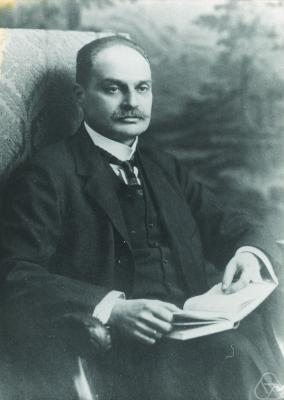
\includegraphics[width=0.76\textwidth,height=4.8cm,keepaspectratio]{../assets/Fritz_Hartogs.jpeg}

\medskip
German mathematician, born in Brussels.

\smallskip
Under the Nazi regime, Hartogs was persecuted as a Jew, forced out of
his professorship, briefly imprisoned in Dachau after the November 1938
pogroms, and died by suicide in 1943.

\smallskip
{\scriptsize Source: Wikipedia, ``Friedrich Hartogs''.}
\end{frame}

\begin{frame}{Step 1: make a smooth extension and measure its error}
Choose $R>0$ with $K\subset B_R$.
Choose a smooth bump function $\chi$ such that
\[
\chi=1\text{ near }K,
\qquad
\operatorname{supp}\chi\subset B_R.
\]
On $\C^n\setminus K$, define
\[
\widetilde f:=(1-\chi)f,
\]
and set $\widetilde f=0$ near $K$.

This is smooth on all of $\C^n$: near $K$ the factor $1-\chi$ is already
zero. Also
\[
\widetilde f=f
\qquad\text{outside }B_R.
\]

Its failure to be holomorphic is
\[
\boxed{\alpha:=\db\widetilde f.}
\]
Because $\widetilde f=f$ outside $B_R$ and $f$ is holomorphic there,
\[
\operatorname{supp}\alpha\subset\overline{B_R}.
\]
Also
\[
\db\alpha=\db^2\widetilde f=0.
\]
\end{frame}

\begin{frame}{Step 2: move the compactly supported error to $\mathbb P^n$}
Identify $\C^n$ with the affine chart
\[
(z_1,\ldots,z_n)\longmapsto[1:z_1:\cdots:z_n]
\]
inside $\mathbb P^n$.
The complement is the hyperplane at infinity
\[
H_\infty=\{Z_0=0\}\cong\mathbb P^{n-1}.
\]

Since $\alpha$ has compact support in $\C^n$, it is zero near
$H_\infty$. Therefore we may extend $\alpha$ by zero and regard it as a
smooth $\db$-closed $(0,1)$-form on all of $\mathbb P^n$.

Now use {\bf (!!!)}
\[
\boxed{H^{0,1}_{\db}(\mathbb P^n)=0.}
\]
Hence there exists a smooth function $\varphi$ on $\mathbb P^n$ such that
\[
\boxed{\db\varphi=\alpha.}
\]

The only remaining problem is: why can we arrange that the correction is
zero far away?
\end{frame}

\begin{frame}{Why $H^{0,1}_{\db}(\mathbb
P^n)=0$ (True, but can we use it?)}
We use two facts already available from Hodge theory:
\begin{enumerate}
\item $\mathbb P^n$ is compact K\"ahler.
\item
\[
H^1_{\mathrm{dR}}(\mathbb P^n,\C)=0.
\]
Indeed, $\mathbb P^n$ has one cell in each even real dimension and no
odd-dimensional cells.
\end{enumerate}

For a compact K\"ahler manifold,
\[
H^1_{\mathrm{dR}}(\mathbb P^n,\C)
\cong
H^{1,0}_{\db}(\mathbb P^n)
\oplus
H^{0,1}_{\db}(\mathbb P^n).
\]
The left-hand side is zero, so both summands are zero. In particular,
\[
\boxed{H^{0,1}_{\db}(\mathbb P^n)=0.}
\]

Thus the equation $\db\varphi=\alpha$ from the previous slide really has
a global smooth solution on $\mathbb P^n$.
\end{frame}

\begin{frame}{Alternative: construct $\varphi$ from $\db$-Poincar\'e}
Cover $\mathbb P^n$ by small polydisks $U_i$.
Since $\alpha$ is $\db$-closed, the $\db$-Poincar\'e lemma gives
local functions
\[
\db\varphi_i=\alpha|_{U_i}.
\]

On overlaps,
\[
\db(\varphi_i-\varphi_j)=0,
\]
so
\[
g_{ij}:=\varphi_i-\varphi_j
\]
is holomorphic. Thus $(g_{ij})$ is a \v Cech $1$-cocycle with values in
$\mathcal O$.

If
\[
H^1(\mathbb P^n,\mathcal O)=0,
\]
then this cocycle is a coboundary:
\[
g_{ij}=h_i-h_j
\]
for holomorphic $h_i$.

Therefore the corrected local primitives
\[
\widetilde\varphi_i:=\varphi_i-h_i
\]
agree on overlaps and glue to a global smooth function $\varphi$ with
\[
\boxed{\db\varphi=\alpha.}
\]
\end{frame}


\begin{frame}{Step 3: the solution is constant outside the ball}
Because $\alpha=0$ outside $\overline{B_R}$,
\(
\db\varphi=0
\) there,
so $\varphi$ is holomorphic there.
Near $H_\infty$, it is also holomorphic. Since
$H_\infty\cong\mathbb P^{n-1}$ is compact and connected,
$\varphi|_{H_\infty}$ is a constant; call it $c$.

Now fix $z\in\C^n$ with $\|z\|>R$.
Because $n\ge2$, through any point $z$
outside the ball {\bf you can choose
a complex line in an extra direction that
stays outside the ball}.
This lets us apply Liouville's theorem to $\varphi$ restricted to that line.

Choose a nonzero complex vector $v$ orthogonal to $z$. Then the complex line
\[
L_z=\{z+tv:t\in\C\}
\]
never meets $\overline{B_R}$, because
\[
\|z+tv\|^2=\|z\|^2+|t|^2\|v\|^2>R^2.
\]

Hence $t\mapsto\varphi(z+tv)$ is an entire bounded function.
By Liouville it is constant, and as $t\to\infty$ it approaches
$H_\infty$, where the value is $c$. Therefore
\[
\boxed{\varphi(z)=c\qquad(\|z\|>R).}
\]
\end{frame}

\begin{frame}{Step 4: subtract the error and finish}
Define
\[
\psi:=\varphi|_{\C^n}-c.
\]
The previous slide says
\[
\psi=0
\qquad\text{outside }\overline{B_R},
\]
so $\psi$ has compact support. Also
\[
\db\psi=\db\varphi=\alpha.
\]

Now set
\[
\boxed{F:=\widetilde f-\psi.}
\]
Then
\[
\db F
=\db\widetilde f-\db\psi
=\alpha-\alpha
=0,
\]
so $F$ is holomorphic on all of $\C^n$.

Outside $B_R$,
\[
\widetilde f=f,
\qquad
\psi=0,
\]
hence $F=f$ there. Since $\C^n\setminus K$ is connected, the identity
theorem gives
\[
F=f\qquad\text{on all of }\C^n\setminus K.
\]

Thus $F$ is the desired extension. Uniqueness follows from the same identity
theorem.
\end{frame}

\end{document}
